%----------------------------------------------------------------------------------------
%	PACKAGES AND THEMES
%----------------------------------------------------------------------------------------

\documentclass{beamer}

\mode<presentation> {

% The Beamer class comes with a number of default slide themes
% which change the colors and layouts of slides. Below this is a list
% of all the themes, uncomment each in turn to see what they look like.

%\usetheme{default}
%\usetheme{AnnArbor}
%\usetheme{Antibes}
%\usetheme{Bergen}
%\usetheme{Berkeley}
%\usetheme{Berlin}
%\usetheme{Boadilla}
%\usetheme{CambridgeUS}
%\usetheme{Copenhagen}
%\usetheme{Darmstadt}
%\usetheme{Dresden}
%\usetheme{Frankfurt}
%\usetheme{Goettingen}
%\usetheme{Hannover}
%\usetheme{Ilmenau}
%\usetheme{JuanLesPins}
%\usetheme{Luebeck}
%\usetheme{Madrid}
%\usetheme{Malmoe}
%\usetheme{Marburg}
%\usetheme{Montpellier}
%\usetheme{PaloAlto}
%\usetheme{Pittsburgh}
%\usetheme{Rochester}
%\usetheme{Singapore}
%\usetheme{Szeged}
\usetheme{Warsaw}

% As well as themes, the Beamer class has a number of color themes
% for any slide theme. Uncomment each of these in turn to see how it
% changes the colors of your current slide theme.

%\usecolortheme{albatross}
%\usecolortheme{beaver}
%\usecolortheme{beetle}
%\usecolortheme{crane}
%\usecolortheme{dolphin}
%\usecolortheme{dove}
%\usecolortheme{fly}
%\usecolortheme{lily}
%\usecolortheme{orchid}
%\usecolortheme{rose}
\usecolortheme{seagull}
%\usecolortheme{seahorse}
%\usecolortheme{whale}
%\usecolortheme{wolverine}

%\setbeamertemplate{footline} % To remove the footer line in all slides uncomment this line
%\setbeamertemplate{footline}[page number] % To replace the footer line in all slides with a simple slide count uncomment this line

%\setbeamertemplate{navigation symbols}{} % To remove the navigation symbols from the bottom of all slides uncomment this line
}

\usepackage{graphicx} % Allows including images
\usepackage{booktabs} % Allows the use of \toprule, \midrule and \bottomrule in tables
\usepackage{listings}
\usepackage{lmodern} 
\setbeamertemplate{footline}[frame number] 
\setbeamertemplate{footline}{%
  \raisebox{5pt}{\makebox[\paperwidth]{\hfill\makebox[10pt]{\scriptsize\insertframenumber\hspace{5pt}}}}}
\beamertemplatenavigationsymbolsempty


\titlegraphic{\vspace{-5em}
\includegraphics[width=2cm]{logoimag.png}\hspace*{4.75cm}~%
   
\includegraphics[width=5cm]{logoujf.pdf}
}
%%%%%%%%%%%%%%%%%%%%%%%%%%%%%%%%%%%%%%%%%
%   TITLE PAGE                          %
%%%%%%%%%%%%%%%%%%%%%%%%%%%%%%%%%%%%%%%%%

\title{Nachos Project}
\subtitle{M1 MOSIG}   
\author{Antoine Faravelon
\\
Lucas Felix
\\
Hugo Guiroux
\\
Miratul Khusna Mufida
\\
Simon Moura
\\
M1 MOSIG, IM$^2$AG UJF 
}
\date{January 2014} 
%%%%%%%%%%%%%%%%%%%%%%%%%%%%%%%%%%%%%%%%%

\begin{document}
\frame{\titlepage} 

\begin{frame}
    %\tableofcontents[sectionstyle=hide/hide, subsectionstyle=show/shaded/hide]
    \tableofcontents
\end{frame}

\begin{frame}{Introduction}
\end{frame}

\section{Features}

\begin{frame}{Main features}
    \begin{itemize}
        \item Input/Output Management
        \item Multi-Threading
        \item Memory Management
        \item File System
        \item Network
    \end{itemize}
\end{frame}

\begin{frame}{Additional Work}
    \begin{itemize}
        \item Socket API 
        \item Dynamic Memory Allocation
        \item User Thread Synchronization (Producer/Consumer)
        \item Process Management (Mini Shell)
        \item Automatic Regression Test 
        \item Absence of memory leak
    \end{itemize}
\end{frame}

\section{Implementation}

\subsection{Multi-Threading}
\begin{frame}{Multi-Threading Model}
    \begin{figure}[ht]
        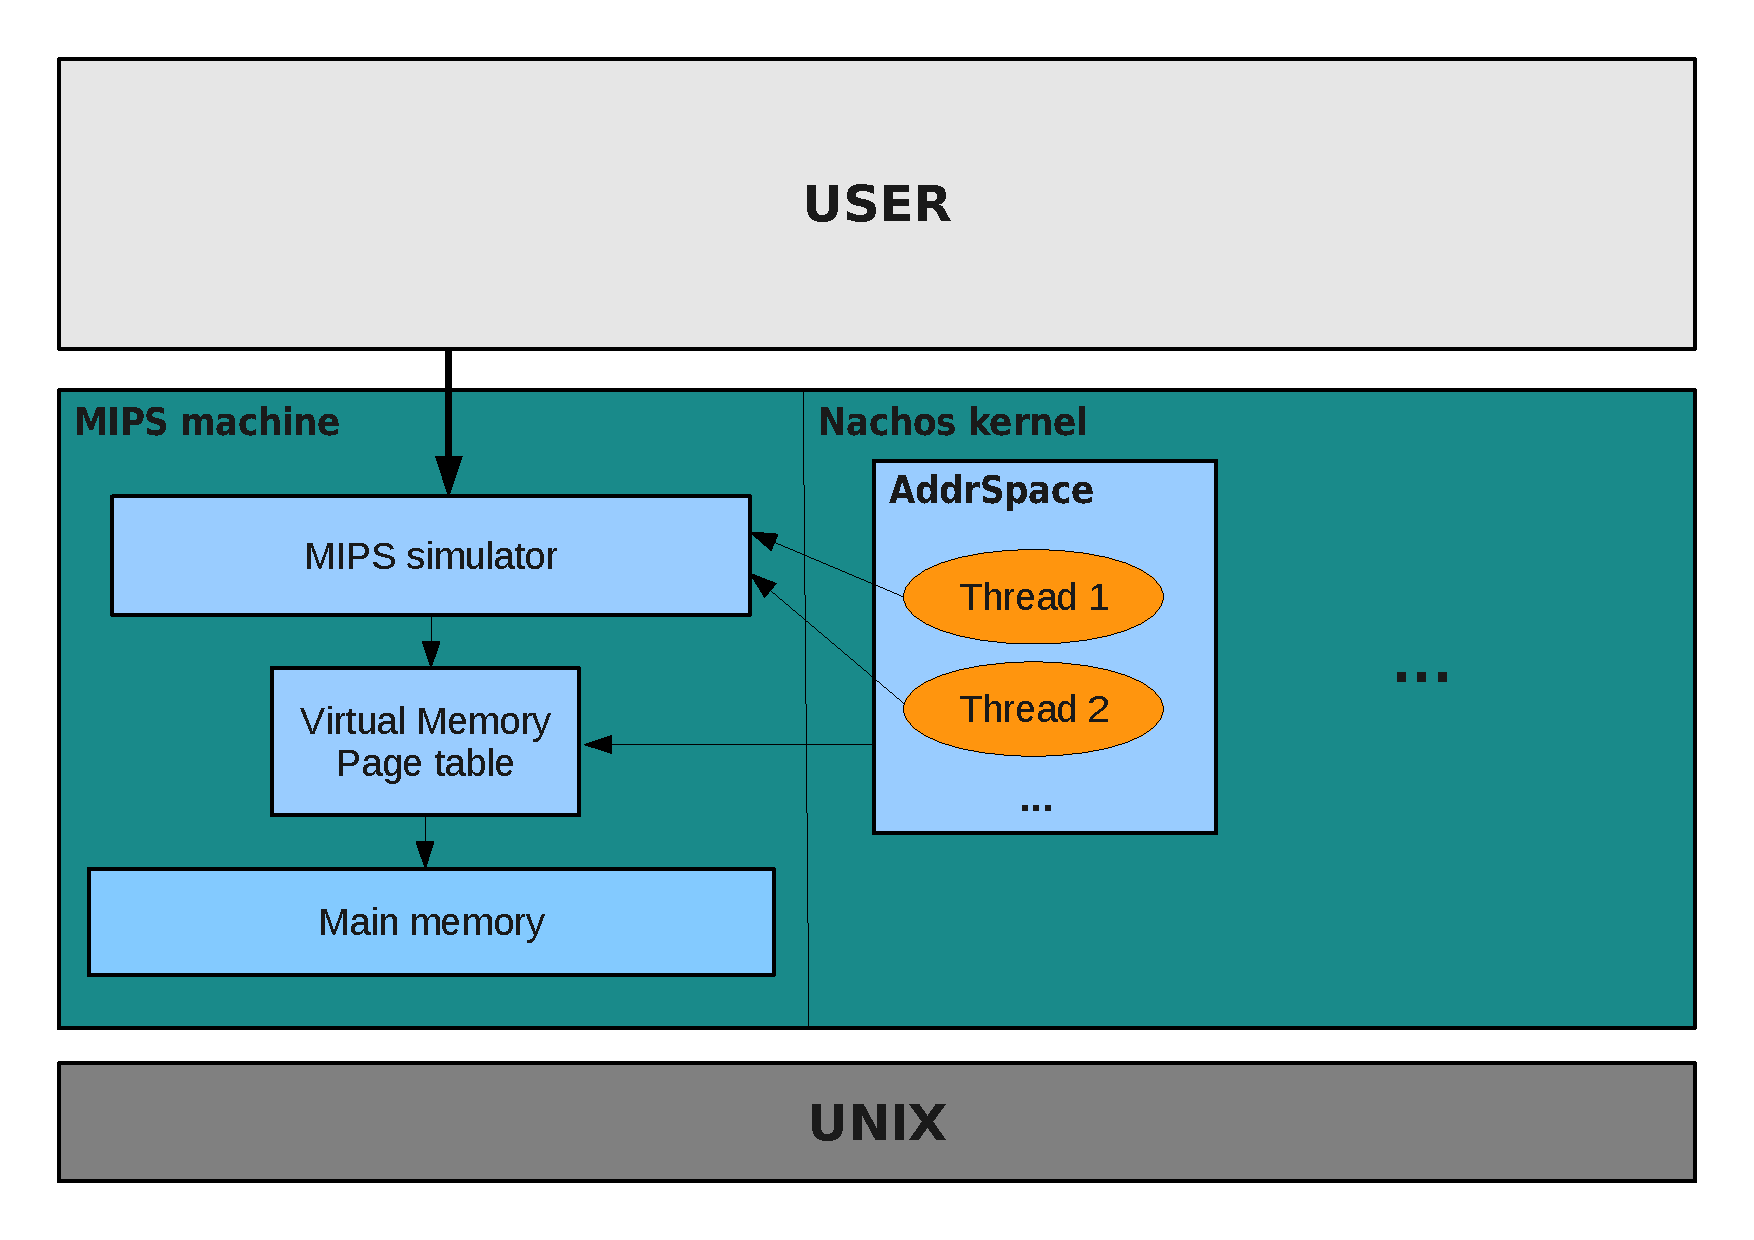
\includegraphics[width=0.8\linewidth]{threadschema.pdf}
    \end{figure}
\end{frame}

\begin{frame}{Multi-Threading issue : Exit Handler}
    \begin{itemize}
        \item Problem : Original thread only execute the specific 
            \\function and return anywhere in the memory 
        \item Solution : Exit Handler
            \begin{itemize}
                \item Explicit Exit (User Thread Exit)
                \item Automatic Exit (Function wrapping)
            \end{itemize}
    \end{itemize}
\end{frame}

\begin{frame}{User Thread Synchronization (Producers/Consumers)}
    \begin{itemize}
        \item Files and folders management
        \item Disk management
    \end{itemize}
\end{frame}

\subsection{Memory Management}
\begin{frame}{Virtual memory management}
    \begin{itemize}
        \item \textbf{Problem :} sharing physical memory between 
            \\processes having multiple threads
        \item \textbf{Solution :}
            \begin{itemize}
                \item Virtual Memory 
                \item Allocate one stack for each thread
            \end{itemize}
    \end{itemize}
\end{frame}

\begin{frame}{Heap/Stack management}
    \begin{figure}[ht]
        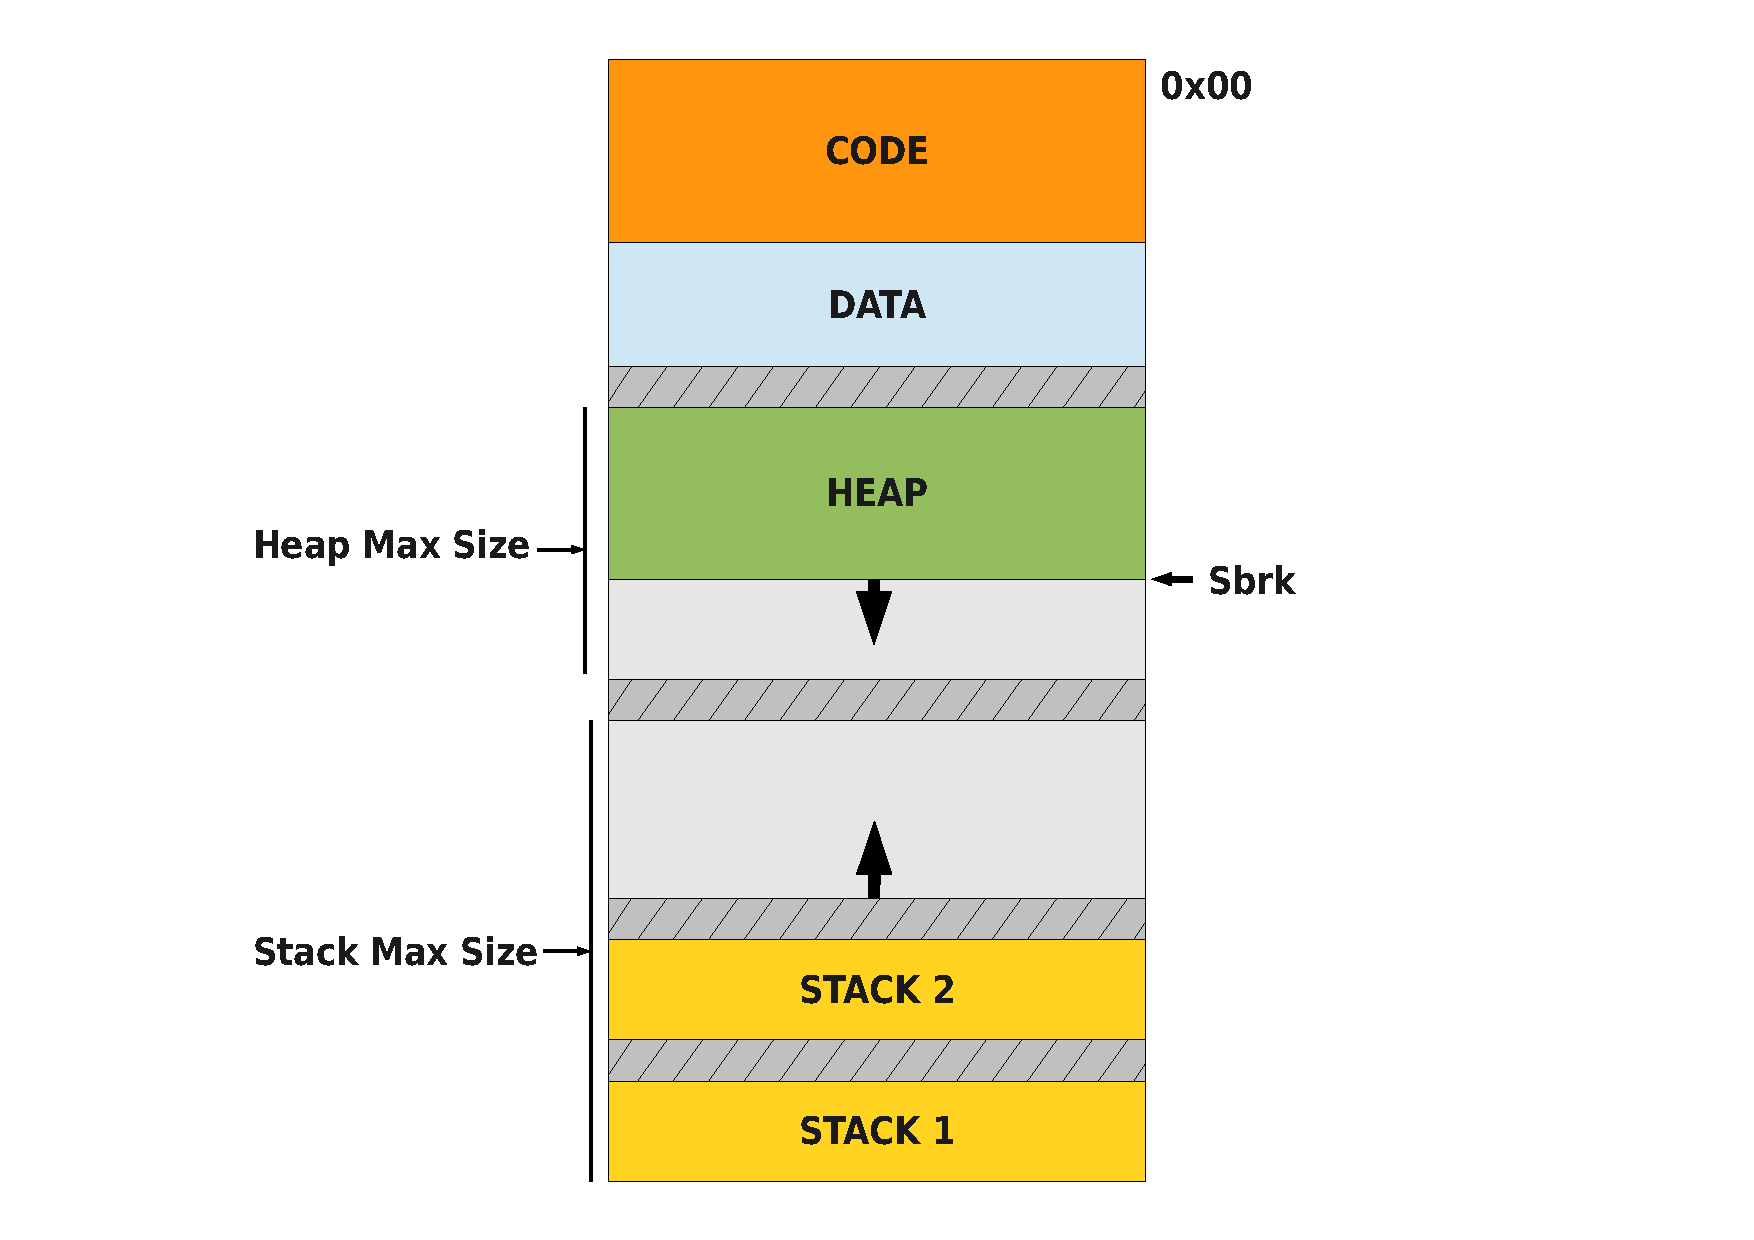
\includegraphics[width=1\linewidth]{memoryschema.pdf}
    \end{figure}
\end{frame}

\subsection{Multi-Process}
\begin{frame}{Multi-Process model}
    \begin{itemize}
        \item Problem : Original code can not handle and
            \\order launching processes
        \item Waitpid Function allows to end the process 
            \\before continue execution of caller another
            \\process to prevent
    \end{itemize}
\end{frame}

\begin{frame}{Process Management (Mini Shell)}
    \begin{itemize}
        \item Files and folders management
        \item Disk management
    \end{itemize}
\end{frame}

\subsection{Network}
\begin{frame}{Network model}
    \begin{figure}[ht]
        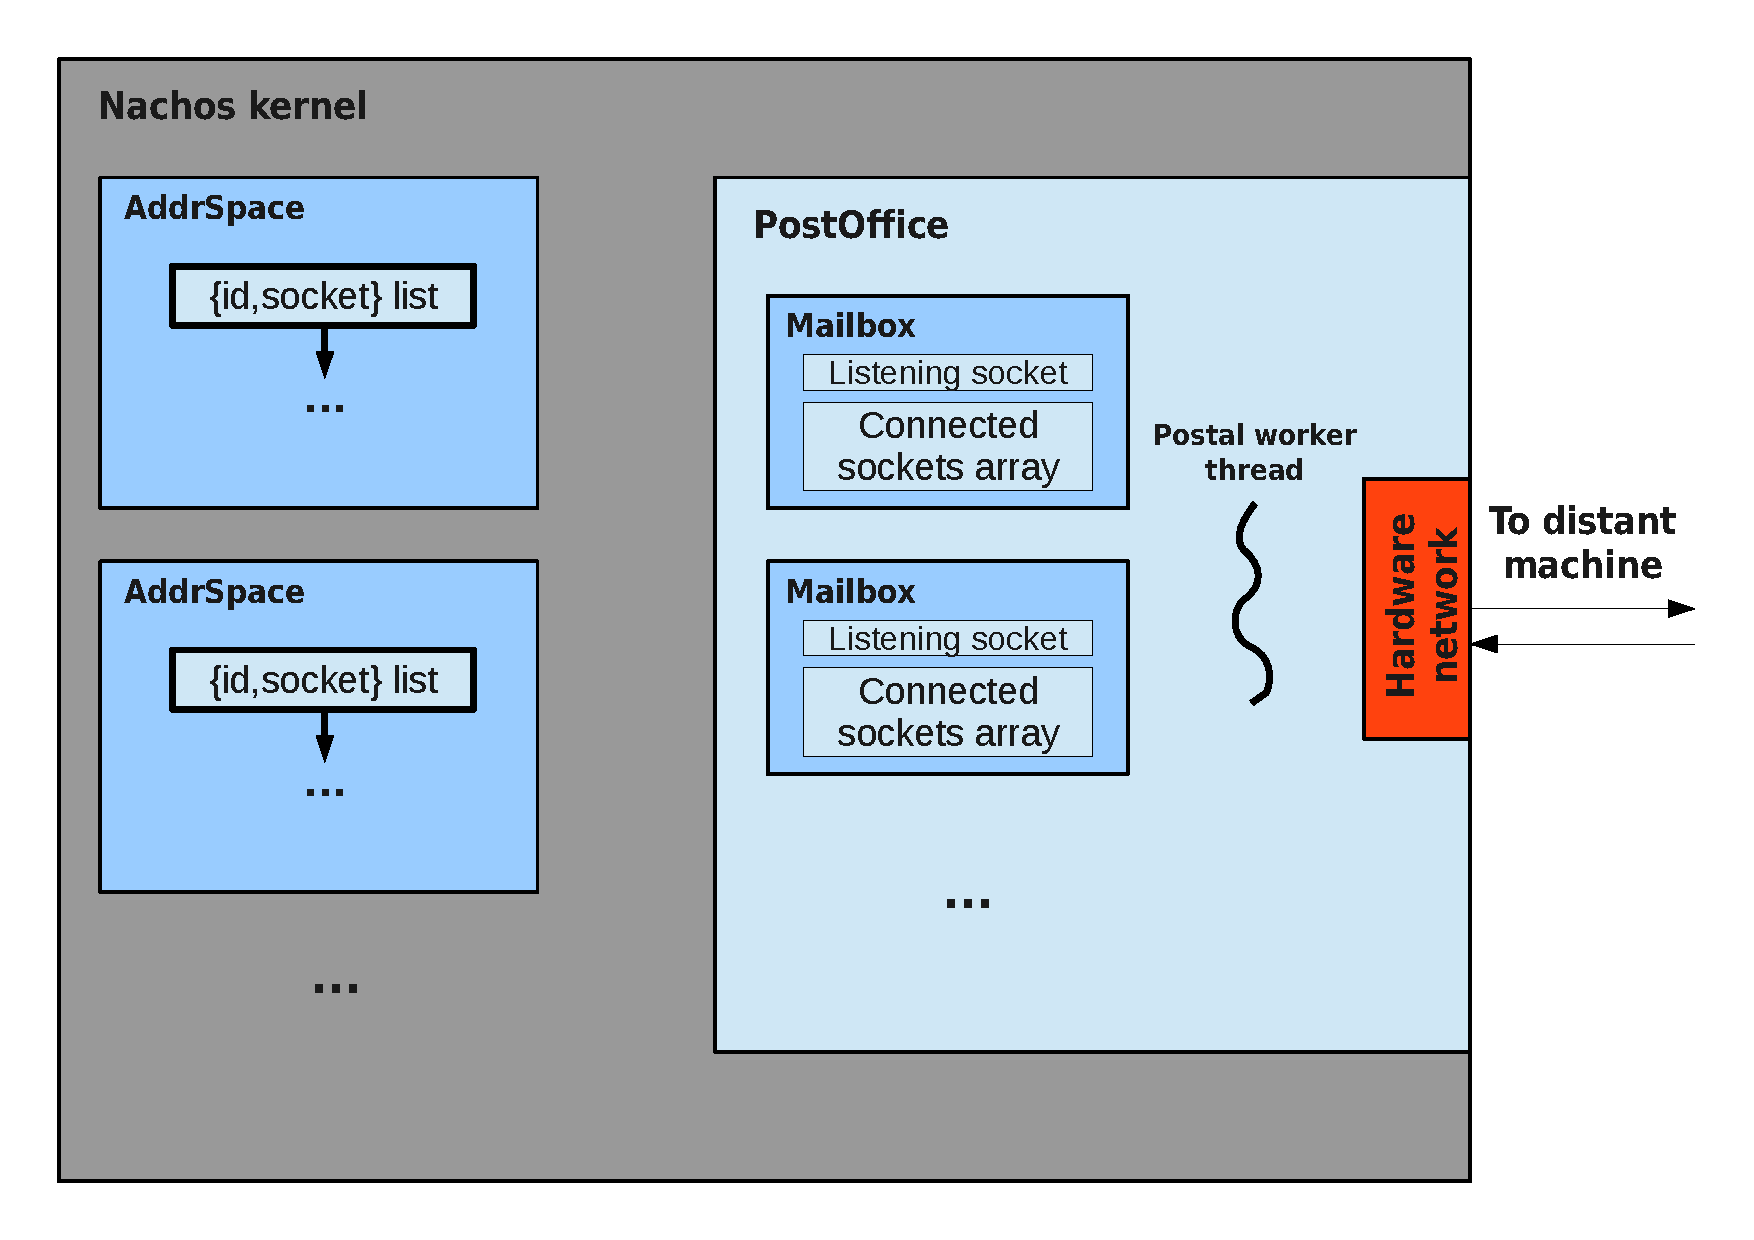
\includegraphics[width=0.7\linewidth]{Networkcolored.pdf}
    \end{figure}
\end{frame}

\begin{frame}{Socket API}
    \begin{itemize}
        \item System calls  
        \item Robust transmission
    \end{itemize}
\end{frame}

\subsection{File system}
\begin{frame}{File system model}
    Schema $-->$ not done yet
\end{frame}

\begin{frame}{Possible extensions}
    \begin{itemize}
        \item \textbf{Robustness} : Journalization techniques
            \begin{itemize}
                \item Log all actions \& replay them if crash
                \item Do write operations in reverse order : only loose of
                    storage space
            \end{itemize}
        \item \textbf{I/O optimization} : elevator algorithm (scheduling minimizing arm
            hard drive moves)
    \end{itemize}
\end{frame}

\section{Quality}
\begin{frame}{Automatic Regression Test}
    \begin{itemize}
        \item Ensure new feature doesn't break previous ones
        \item Set of $132$ tests
        \item Test all cases we could imagine
        \item Helped removing bugs/memory leak
        \item Almost no debug phase
    \end{itemize}
\end{frame}

\begin{frame}{Memory leak prevention}
    \begin{itemize}
        \item No more memory leak
        \item System well tested
        \item No bad memory access
        \item Patch for Valgrind/Nachos provided
    \end{itemize}
\end{frame}

\section{Project Management}
\begin{frame}{Team work}
    \begin{itemize}
        \item Every day at university
        \item Teams of 2 or 3
        \item Extreme programming
        \item Test driven development
        \item GIT
    \end{itemize} 
\end{frame}

\begin{frame}{Conclusion}
    \textbf{Missing features :}
    \begin{itemize}
        \item Network : process migration, multi-threading support
        \item File system : I/O optimization \& robustness
    \end{itemize}

    \textbf{Strong points :}
    \begin{itemize}
        \item No memory leak
        \item Almost all bonuses done (missing 2)
        \item Substantial set of tests
        \item Socket API
    \end{itemize}
\end{frame}

\end{document}
